Если бы в атоме гелия электроны взаимодействовали друг с другом, а только с ядром, то мы бы получили водородоподобный атом с $Z = 2$ и энергией отрыва одного электрона (однократная ионизация) была бы равна 
\begin{equation*}
	\frac{m e^4 Z^2}{2 \hbar^2} \frac{1}{1^2} = 13.6 \cdot 4 = 54.4 \text{ эВ}.
\end{equation*}
Экспериментальное значение $24.9$ эВ. Причина расхождения -- неучёт  кулоновского отталкивания электронов.

Будем считать кулоновское отталкивание "малым". Как видно из вышеприведенного примера это не так. Поэтому дальнейшее надо рассматривать, как в основном качественный подход.

В отсутствии взаимодействия основное состояние есть состояния $1s$ с энергией $-54.4$ эВ согласно принципу Паули мы можем поместить в это состояние 2 электрона только если их спины будут противоположны (-$\uparrow$-$\downarrow$-).
Следовательно $(S_z)_\text{max} = 0$ и поскольку других вариантов нет, то и $S = 0$.  

Это антисимметричное по спину состояние, поэтому орбитальное состояние должно быть симметричным
\begin{equation*}
	\varphi(1,2) = \frac{\varphi_{1s}(1) \varphi_{1s}(2) + \varphi_{1s}(2) \varphi_{1s}(1)}{\sqrt{2}} = \sqrt{2} \varphi_{1s}(1) \varphi_{1s}(2),
\end{equation*}
где $\varphi_{1s}(\vc{r}) = \frac{Z^{3/2}}{\sqrt{\pi a_B^3}} e^{- Z r/a_B}$ -- волновая функция электрона в состоянии $1s$ в поле заряда $Z e$.

Найдём средние значение кулоновского отталкивания электронов в этом состоянии
\begin{align*}
	\langle \hat{V}_\text{кул} \rangle &= \iint d v_1 d v_2 \varphi^*(1,2) \frac{e^2}{|\vc{r}_1 - \vc{r}_2|}\varphi(1,2)\\
	&=
	\iint d v_1 d v_2 \varphi^*_{1s}(1) \varphi^*_{1s}(2) \frac{e^2}{|\vc{r}_1 - \vc{r}_2|} \varphi_{1s}(1) \varphi_{1s}(2)\\
	&=
	\iint d v_1 d v_2 \frac{e |\varphi_{1s}(1)|^2 \cdot e |\varphi_{1s}(2)|^2}{|\vc{r}_1 - \vc{r}_2|}
	= \iint \frac{\rho_{1s}(1) \rho_{1s}(2)}{|\vc{r}_1 - \vc{r}_2|} d v_1 d v_2,
\end{align*}
где $\rho_{1s}(1) = e |\varphi_{1s}(1)|^2$ -- плотность заряда электронного облака 1-го электрона в состоянии $1s$; $\rho_{1s}(2)$ -- аналогично для 2-го электрона. Так как
\begin{equation*}
	p_{1s}(1) dv_1 = d q_1,
	\hspace{1 cm}
	\rho_{1s}(2) d v_2 = d q_2,
\end{equation*}
и мы получаем классическое выражение для энергии кулоновского отталкивания объёмных (не точеных!!!) зарядов.
Вычисление интеграла с волновыми функциями $1s$-состояния даёт (см. задачу $\boxed{4.48}$)
\begin{equation*}
	E_\text{кул} = \langle \hat{V}_\text{кул}\rangle = \frac{5}{8} \frac{Z e^2}{a_\text{Б}} = 34 \text{эВ}.
\end{equation*}

Причина расхождения с экспериментальными данными ($54.4 - 24.9 = 29.5$ эВ) состоит в том, что находящиеся в состоянии $1s$ электроны могут подходить близко к ядру и частично "закрывать" своим электронным облаком (экранировать) поле заряда $+2e$.
В результате электроны "чувствуют" уменьшенный заряд ядра. 
Теоретический расчет показывает, что $Z_\text{эфф} = Z - \frac{5}{16}$ и $E_\text{кул} = 28.7$ эВ, что уже близко к эксперименту.

Теперь рассмотрим возбужденное состояния атома гелия. Для этого нужно перевести один из электронов в состояние $2s$ (в модели невзаимодействующих электронов есть ещё уровень $2p$ с той же энергией).

% \begin{wrapfigure}{r}{0.2\textwidth}
% 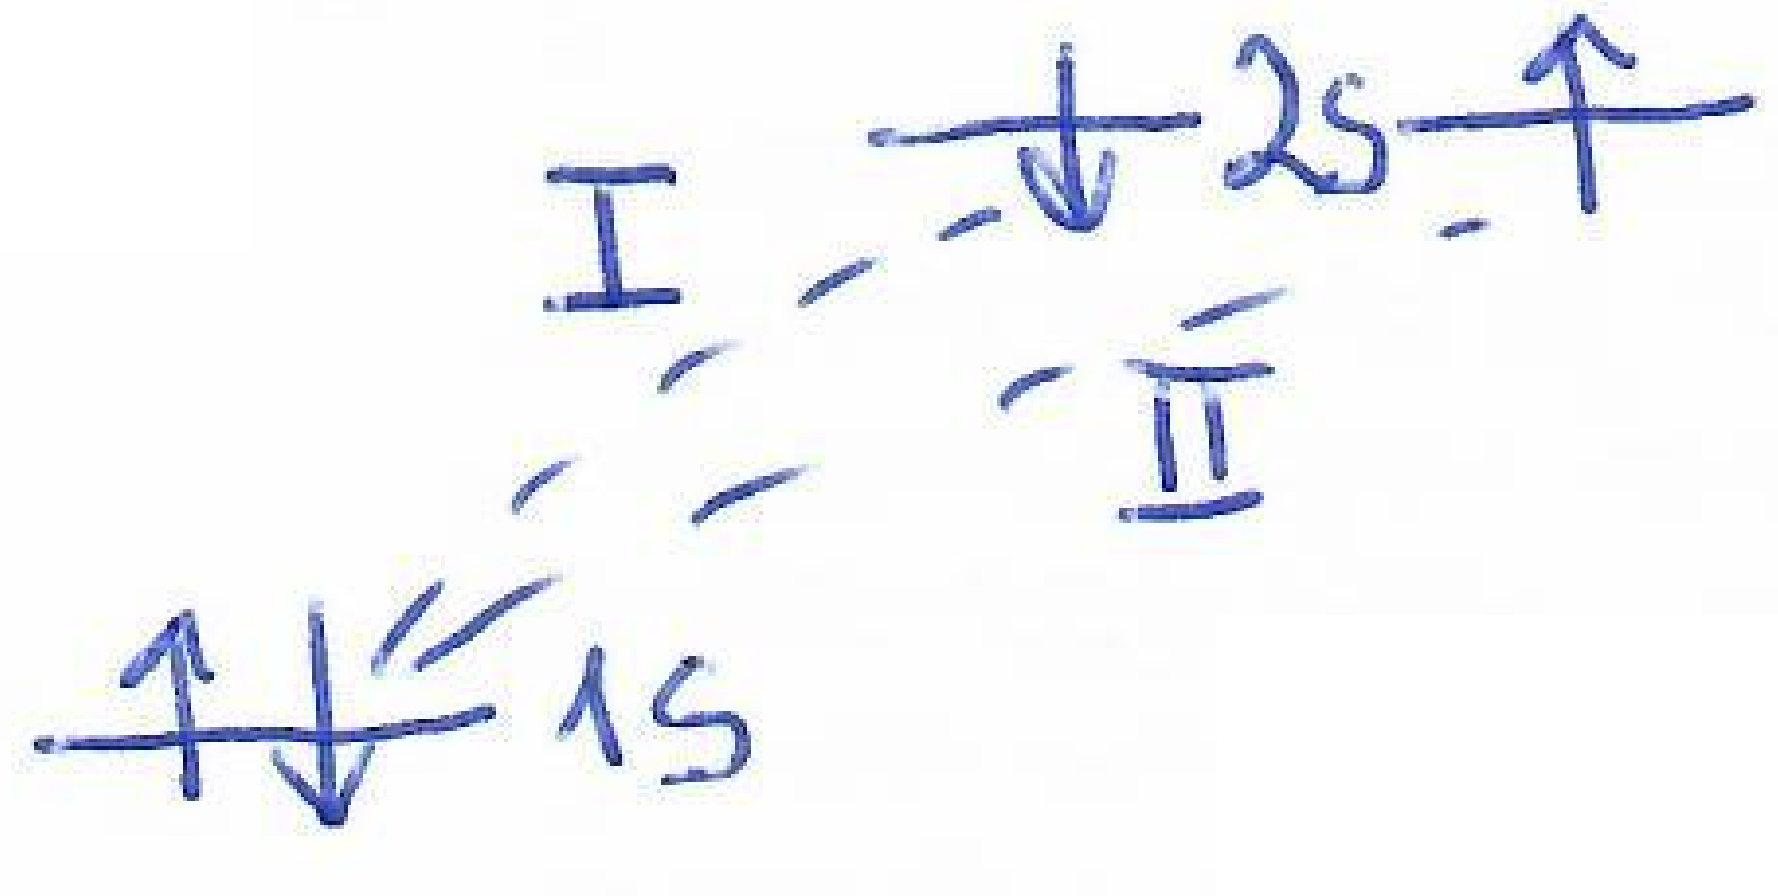
\includegraphics[width=0.2\textwidth]{image/1sto2s.png}
% \end{wrapfigure}
\begin{minipage}{0.33\textwidth}
    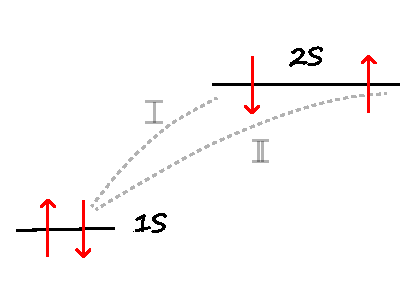
\includegraphics[width=1\textwidth]{image/1sto2s.pdf}
\end{minipage}
\hfill
\begin{minipage}{0.6\textwidth}
    Однако его можно перевести так, чтобы суммарный спин остался равным $0(I)$ или стал равным $1(II)$.

	Соответственно среднее значение кулоновского отталкивания будет разным.
\end{minipage}

\begin{align*}
	\langle \hat{V}_\text{кул}\rangle 
	=
	\iint dv_1 dv_2 \big( [\varphi_{1s}^*(1) \psi_{2s}^*(2) \pm &\varphi_{1s}^*(2) \psi_{2s}^*(1)]
	\frac{e^2}{|\vc{r}_1 - \vc{r}_2|} \frac{1}{\sqrt{2}} \cdot
	\\
	&\cdot\frac{1}{\sqrt{2}}
	[\varphi_{1s}(1) \psi_{2s}(2) \pm \varphi_{1s}(2) \psi_{2s}(1)]\big).
\end{align*}
Здесь 
\begin{equation*}
	\varphi_{1s}(r) = \frac{Z^{3/2}}{\sqrt{\pi a_\text{Б}^3}} e^{- Z r/a_\text{Б}}, 
	\hspace{0.5 cm}
	\psi_{2s}(r) =  \frac{Z^{3/2}}{2\sqrt{\pi a_\text{Б}^3}} e^{- Z r/a_\text{Б}} \left(1 - \frac{Z r}{2 a_\text{Б}}\right).
\end{equation*}
\begin{figure}[h]
    \centering
    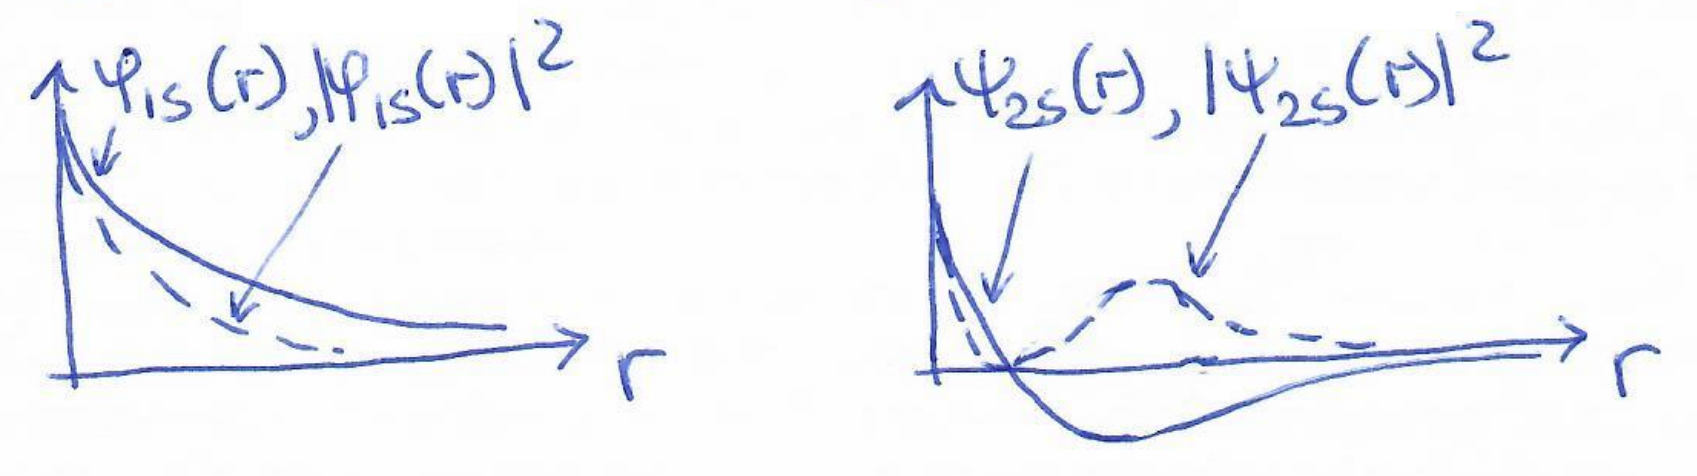
\includegraphics[width=0.9\textwidth]{image/fi1sfi2s.png}
    %\caption{}
    %\label{fig:}
\end{figure}
\begin{align*}
	\langle &\hat{V}_\text{кул}\rangle 
	=
	\frac{1}{2}
	\iint dv_1 dv_2
	\big[
	|\varphi_{1s}(1)|^2 |\psi_{2s}(2)|^2 + |\varphi_{1s}(2)|^2 |\psi_{2s}(1)|^2
	\big] \frac{e^2}{|\vc{r}_1 - \vc{r}_2|} \pm
	\\
	&\pm 
	\frac{1}{2}
	\iint dv_1 dv_2
	\big[
	\varphi_{1s}^*(1) \varphi_{1s}(2) \psi_{2s}^*(2) \psi_{2s}(1) 
	+ 
	\varphi_{1s}^*(2) \varphi_{1s}(1) \psi_{2s}^*(1) \psi_{2s}(2)
	\big] \frac{e^2}{|\vc{r}_1 - \vc{r}_2|}.
\end{align*}

Поскольку по координатам обоих электронов идёт интегрирование, то вклады двух слагаемых в верхней и нижней строчках одинаковы.
В этом легко убедиться, поменяв индексы местами: $\iint dv_1 dv_2 = \iint dv_1 dv_2$. Тогда
\begin{equation*}
	\langle \hat{V}_\text{кул}\rangle 
	= 
	\iint \frac{e |\varphi_{1s}(1)|^2 e|\psi_{2s}(2)|^2}{|\vc{r}_1 - \vc{r}_2|} dv_1 dv_2
	\pm
	\iint \frac{ e\varphi_{1s}^*(1) \varphi_{1s}(2) e \psi_{2s}^*(2) \psi_{2s}(1) }{|\vc{r}_1 - \vc{r}_2|} dv_1 dv_2.
\end{equation*}
Первый член -- не что иное, как классическое кулоновское отталкивание двух электронных облаков $1s$ и $2s$. А вот второй член -- это чисто вантовый эффект отталкивания "обменных" плотностей зарядов $e \varphi_{1s}^*(2) \psi_{2s}(1)$ и $e \psi_{2s}^*(2) \varphi_{1s}(2)$.
Электроны как бы меняются "местами", точнее состояниями.

При нашем рассмотрении $\varphi_{1s}$ и $\psi_{2s}$ -- действительные величины (поскольку нет зависимости от углов) и написание $\varphi_{1s}^*$ и $\psi_{2s}^*$ не более чем дань традиции.
Для других состояний с $l\neq 0$ второй интеграл так же положителен.

$\langle \hat{V}_\text{кул}\rangle = E_\text{кул}^\text{класс} \pm E_\text{кул}^\text{квант}$.
Знак "плюс" соответствует $S = 0$, знак "минус" соответствует полному спину $S=1$.
В первом случае отталкивание сильнее, так как принцип паули "не мешает"  электронам подойти близко друг к другу (спины антипараллельны).
Во втором случае спины параллельны и принцип Паули "мешает" электронам сблизиться и они отталкиваются слабее, чем в первом случае.
Картина энергетических уровней атому выглядит так:
\begin{figure}[h]
    \centering
    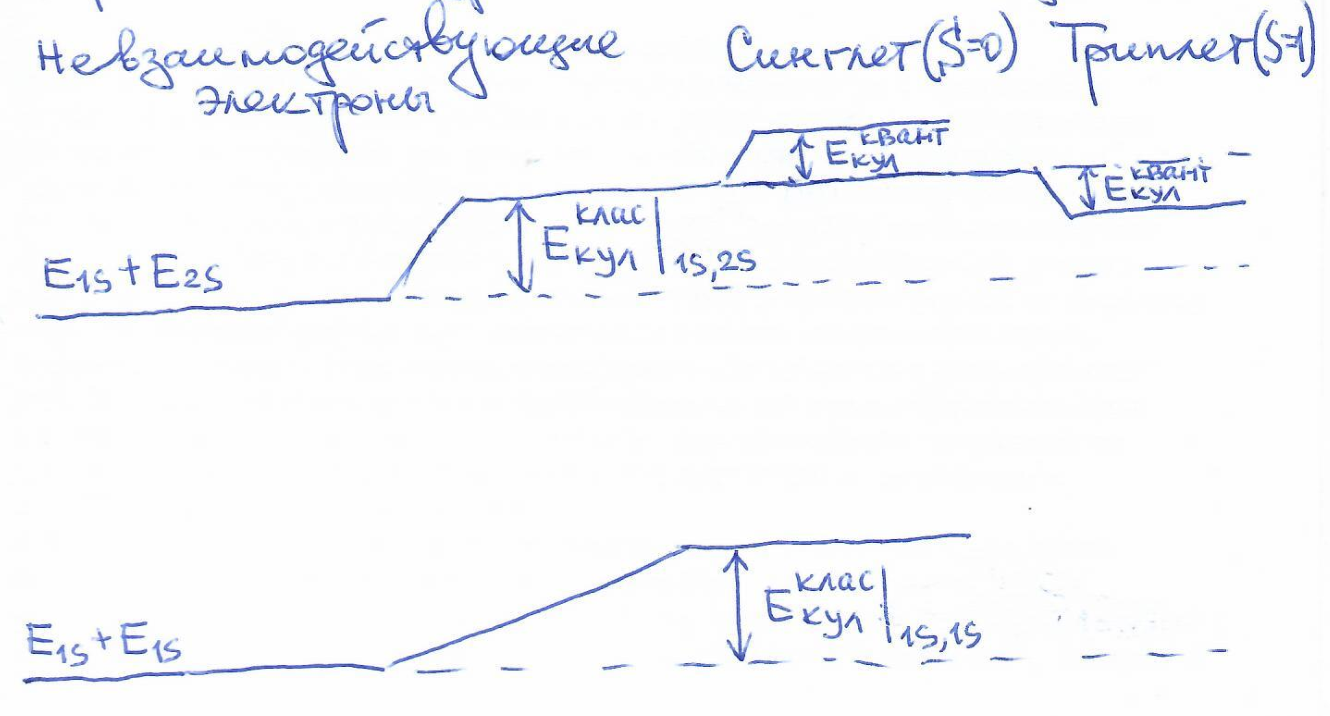
\includegraphics[width=0.8\textwidth]{image/singlr_tripl.png}
    %\caption{}
    %\label{fig:}
\end{figure}


Применим это к задаче $\boxed{6.78}$, но сначала терминология.
Гелий в синглетных состояниях называется парагелий, в триплетных -- ортогелий. 
Синглет -- потому что у спина $0$ есть только одна проекция (single).
Триплет -- потому что у спина $1$ три проекции (triple).

Если не учитывать экранирование и считать электроны изначально невзаимодействующими, то
\begin{equation*}
	\begin{aligned}
		&E_{1s} = - \frac{m e^4}{2 \hbar} \frac{2^2}{1^2} = -54.4 \text{ эВ}\\
		&E_{2s} = - \frac{m e^4}{2 \hbar} \frac{2^2}{2^2} = -13.6 \text{ эВ}
	\end{aligned}
	\hspace{0.3 cm}
	\leadsto
	\hspace{0.3 cm}
	E_{1s} + E_{2s} = - 68 \text{ эВ}.
\end{equation*}

Полная энергия ионизации
\begin{equation*}
	\left\{
	\begin{aligned}
		&W_\text{орто} = - (E_{1s} + E_2s) - E_\text{кул}^\text{класс}\big|_{1s,2s} + E_\text{кул}^\text{квант}\\
		&W_\text{пара} = - (E_{1s} + E_{2s})
		- E_\text{кул}^\text{класс} \big|_{1s,2s} - E_\text{кул}^\text{квант}
	\end{aligned}
	\right.
\end{equation*}
Откуда
\begin{align*}
	&E_\text{кул}^\text{квант} = \frac{W_\text{орто} - W_\text{пара}}{2} = 0.4 \text{ эВ}\\
	&E_\text{кул}^\text{класс}\big|_{1s,2s} = \frac{-2 (E_{1s} + E_{2s}) - W_\text{орто}- W_\text{пара}}{2} = 9.2 \text{ эВ}
\end{align*}
Для дальнейшего следует отметить, что полученный результат отнюдь не мал и не содержит релятивистской малости (не содержит $1/c$ и $1/c^2$). 

Для всех остальных возбужденных состояний $1s^1 n p^1, 1s^1 n d^1$ и т.д. картина будет аналогичной: "\textit{триплет лежит ниже синглета}".
Правда $E_\text{кул}^\text{квант}$ будет уменьшаться.
Причина очевидна: "обменяться состояниям" электроны могут только, если хи волновые функции перекрываются в пространстве -- обмен идут через область перекрытия.

Учёт релятивистских поправок (см. другую часть семинара) приведет к тонкой структуре триплета.

Разобранная задача впервые была решена Гейзенбергом, который объяснил наблюдавшиеся особенности в спектре гелия: он состоит из двух серий, отличающихся по длине волны. 
Одна из серий переходы между синглетными подуровнями, а другая -- между триплетными. 
Дело в том, что при электромагнитных переходах спин состояния не меняется. 
Практически в в спектре гелия есть только одна линия перехода между синглетом и триплетом (так называемая интеркомбинационная линия).

До работы Гейзенберга думали, что в природе есть два разных гелия. Но оказалось, что все таки один!

Впоследствии Дирак предложил записывать синглетно-триплетное расщепление, как среднее значение оператора обменного взаимодействия
\begin{equation*}
	\hat{V}_\text{обм} = -\frac{A}{2}(1+4 \vc{\hat{S}}_1 \vc{\hat{S}}_2).
\end{equation*}

Тогда энергия обменного взаимодействия для случая синглета ($\vc{S} = \vc{S}_1 + \vc{S}_2$) есть
\begin{equation*}
	\langle \hat{V}_\text{обм}\rangle = -\frac{A}{2}(1 + 4 \langle \vc{\hat{S}}_1 \vc{\hat{S}}_2\rangle) = - \frac{A}{2}\left(1 + 4 \left\langle \frac{\vc{S}^2 - \vc{S}_1^2 - \vc{S}_2^2}{2}\right\rangle\right),
\end{equation*}
раньше $S_1$ и $S_2$ -- прецессировали  независимо относительно оси квантовая и интегралами движения были $S_1^2 S_{1z} S_2^2 S_{2z}$.
После включения взаимодействия интегралами движения станут $S^2S_{z}S_1^2S_2^2$, и $S_1$ и $S_2$ будет прецессировать вокруг $\vc{S}$, а $\vc{S}$ -- вокруг оси квантования. Тогда
\begin{minipage}{0.3\textwidth}
    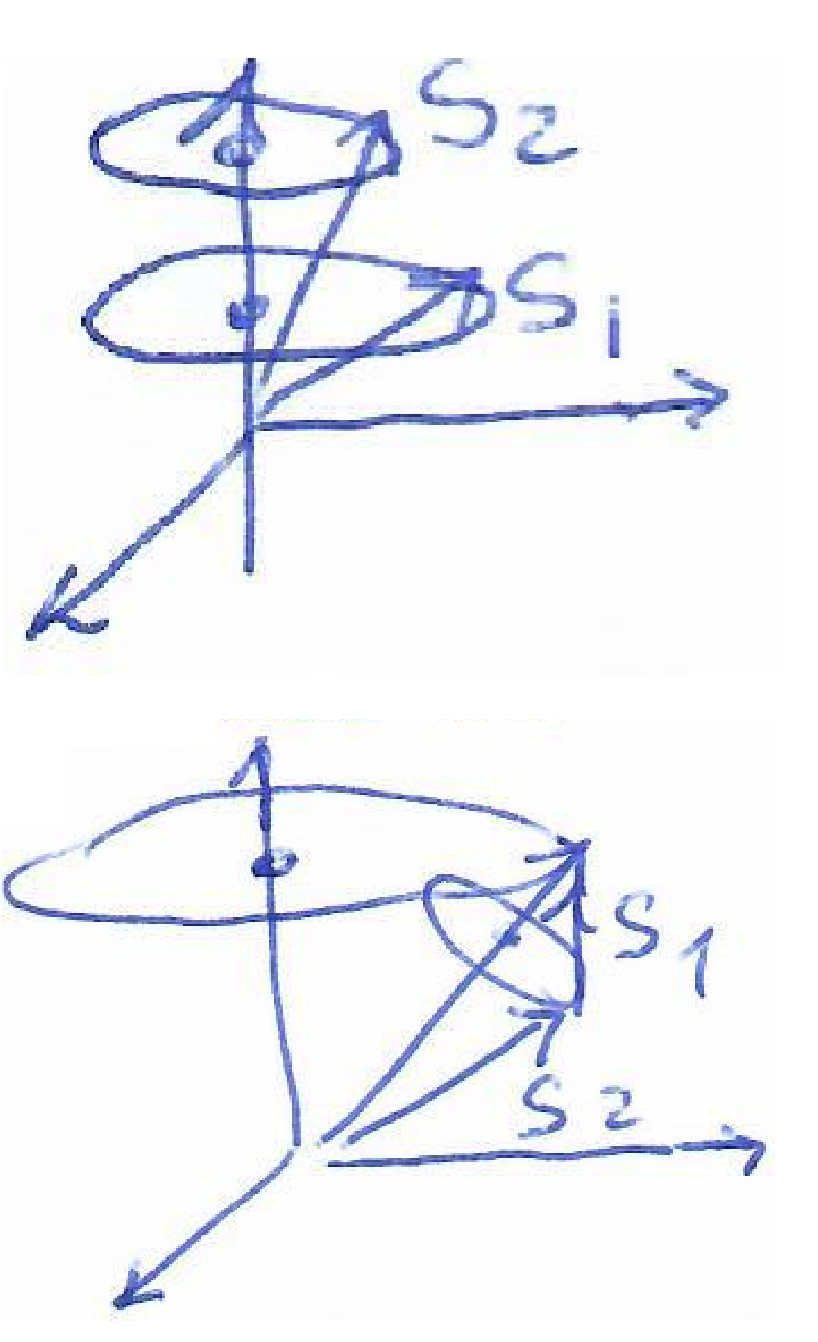
\includegraphics[width=0.9\textwidth]{image/s1-s1.png}
\end{minipage}
\hfill
\begin{minipage}{0.666\textwidth}
	\begin{equation*}
		\left\langle\vc{S}^2 - \vc{S}_1^2 - \vc{S}_2^2\right\rangle
		= S(S+1) - S_1 (S_1 +1) - S_2(S_2+1)
	\end{equation*}    
	\begin{equation*}=\left\{
		\begin{aligned}
			1\cdot 2 - \frac{1}{2}\cdot \frac{3}{2} - \frac{1}{2}\cdot \frac{3}{2} = \frac{1}{2}, \, S = 1\\
			0\cdot 1- \frac{1}{2}\cdot \frac{3}{2} - \frac{1}{2}\cdot \frac{3}{2} = -\frac{3}{2}, \, S=0
		\end{aligned}
		\right.
	\end{equation*}
	\begin{equation*}
	\langle \hat{V}_\text{обм}\rangle = - \frac{A}{2} \left\{
	\begin{aligned}
		1+ \frac{4}{2} \cdot \frac{1}{2} = - A, \, S=1\\
		1 - \frac{4}{2}\cdot \frac{3}{2} = +A, \, S = 0
	\end{aligned}
	\right.
\end{equation*}
\end{minipage}
Сравнивая с решением задачи про спектр получаем $A = E_\text{кул}^\text{квант} > 0$.

Величина $A$ носит название обменной константы (обменного интеграла) и при $A>0$ энергетически выгоднее триплет, то есть параллельное расположение спинов.
При $A<0$ будет выгоднее антипараллельное расположение.
Такой подход используется в теории магнетизма, где оператор $\hat{V}_\text{обм}$ носит название гамильтониана Гейзенберга.

Ещё раз подчеркнём, что никакого особого взаимодействия под названием "обменное" в природе нет!!!
Просто это обозначение квантовой добавки к среднему значению кулоновского (то есть электромагнитного) взаимодействия.
Эта добавка есть следствие учета правильной перестановочной симметрии полных волновых функций.

